\section{Formalization of Knowledge}

\subsection{Abstraction of Methodological, Conceptual, and Factual Knowledge}

The most abstract level of knowledge, methodological knowledge, describes the formalisms through which knowledge can be represented.
The two most common schemata for methodological knowledge are \ac{RDFS} and \ac{OWL}.
They provide the faculty to describe the middle level, conceptual knowledge, which encodes the classes, relations, and constraints relevant to a given domain.
The most common conceptual knowledge formats in the biomedical domain are \ac{BioPAX}, \ac{SBML}, and \ac{BEL}.
The most concrete level is factual knowledge, which consists of instances of these classes and relationships~\cite{Marchetti2008}.
These abstractions are illustrated in Figure~\ref{fig:knowledge_types}.

\begin{figure}
    \captionsetup{format=plain}
    \makebox[\textwidth]{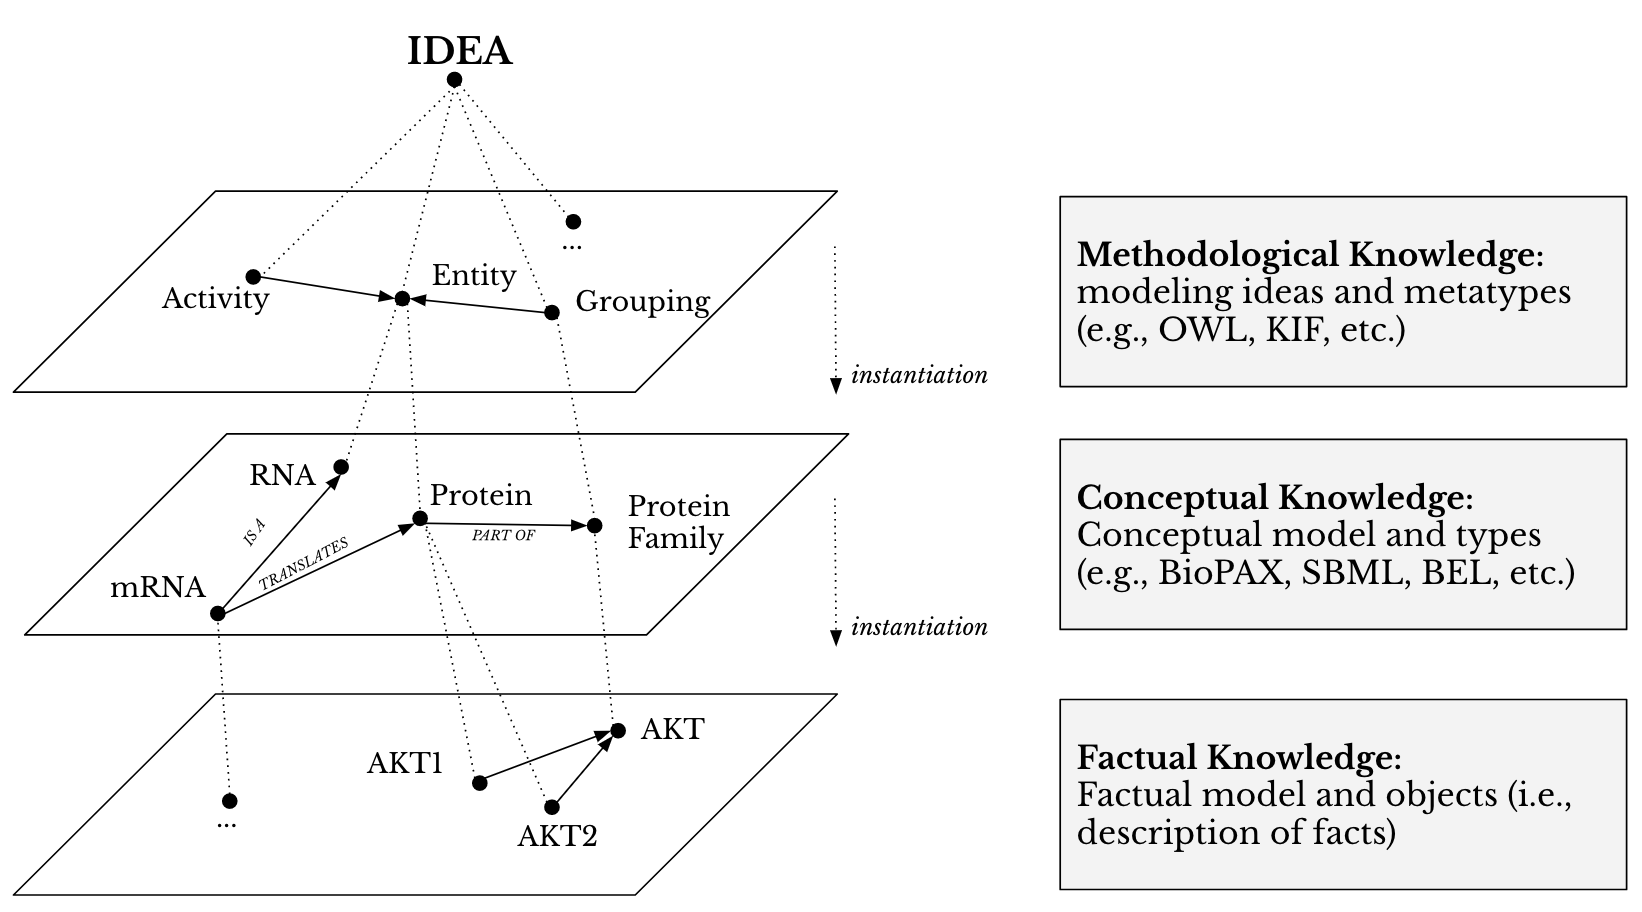
\includegraphics[width=160mm]{figures/knowledge_types.png}}
    \caption[Levels of Knowledge Abstraction]{The interplay of the three levels of knowledge abstraction in an example from the biological domain. This figure can be cited directly with~\cite{Hoyt2019KnowledgeLevels}.}
    \label{fig:knowledge_types}
\end{figure}

\subsection{Realizations}

\subsubsection{Resource Description Framework Schema}

\ac{RDF} uses triples of subjects, predicates, and objects to represent relations between concepts.
Each resource in a triplet is backed by an \ac{IRI}.
While its simple format grants it expressive power, \ac{RDF} lacks structure or domain specificity.
\ac{RDFS} is a set of concepts and predicates appropriate for describing knowledge at the conceptual level.
Included are predicates for asserting class hierarchies (rdfs:subClassOf), asserting memberships (rdf:type), describing the domain and range of predicates (rdfs:domain, rdfs:range), and representing epistemological concepts such as classes, literals, and other data types~\cite{Beckett2014}.
RDF and RDFS are supported by most popular programming languages with packages to serialize and deserialize RDF in a variety of formats (e.g., \ac{XML}, N-Triples, turtle, etc.) and reason over \ac{RDFS}.

\subsubsection{Web Ontology Language}

Like \ac{RDFS}, \ac{OWL} consists of the methodological knowledge for modeling domain-specific knowledge.
Its most simple form, \ac{OWL} Lite, enables the representation of classes, their properties, relations, and constraints.
The most common form, \ac{OWL} \ac{DL}, contains the additional expressive power of descriptive logic over which inferences can be made.
The most expressive form, \ac{OWL} Full, removes the remaining restrictions on \ac{OWL} \ac{DL} but paradoxically becomes undecidable and hinders automatic reasoning~\cite{Marchetti2008}.

\begin{figure}
    \captionsetup{format=plain}
    \makebox[\textwidth]{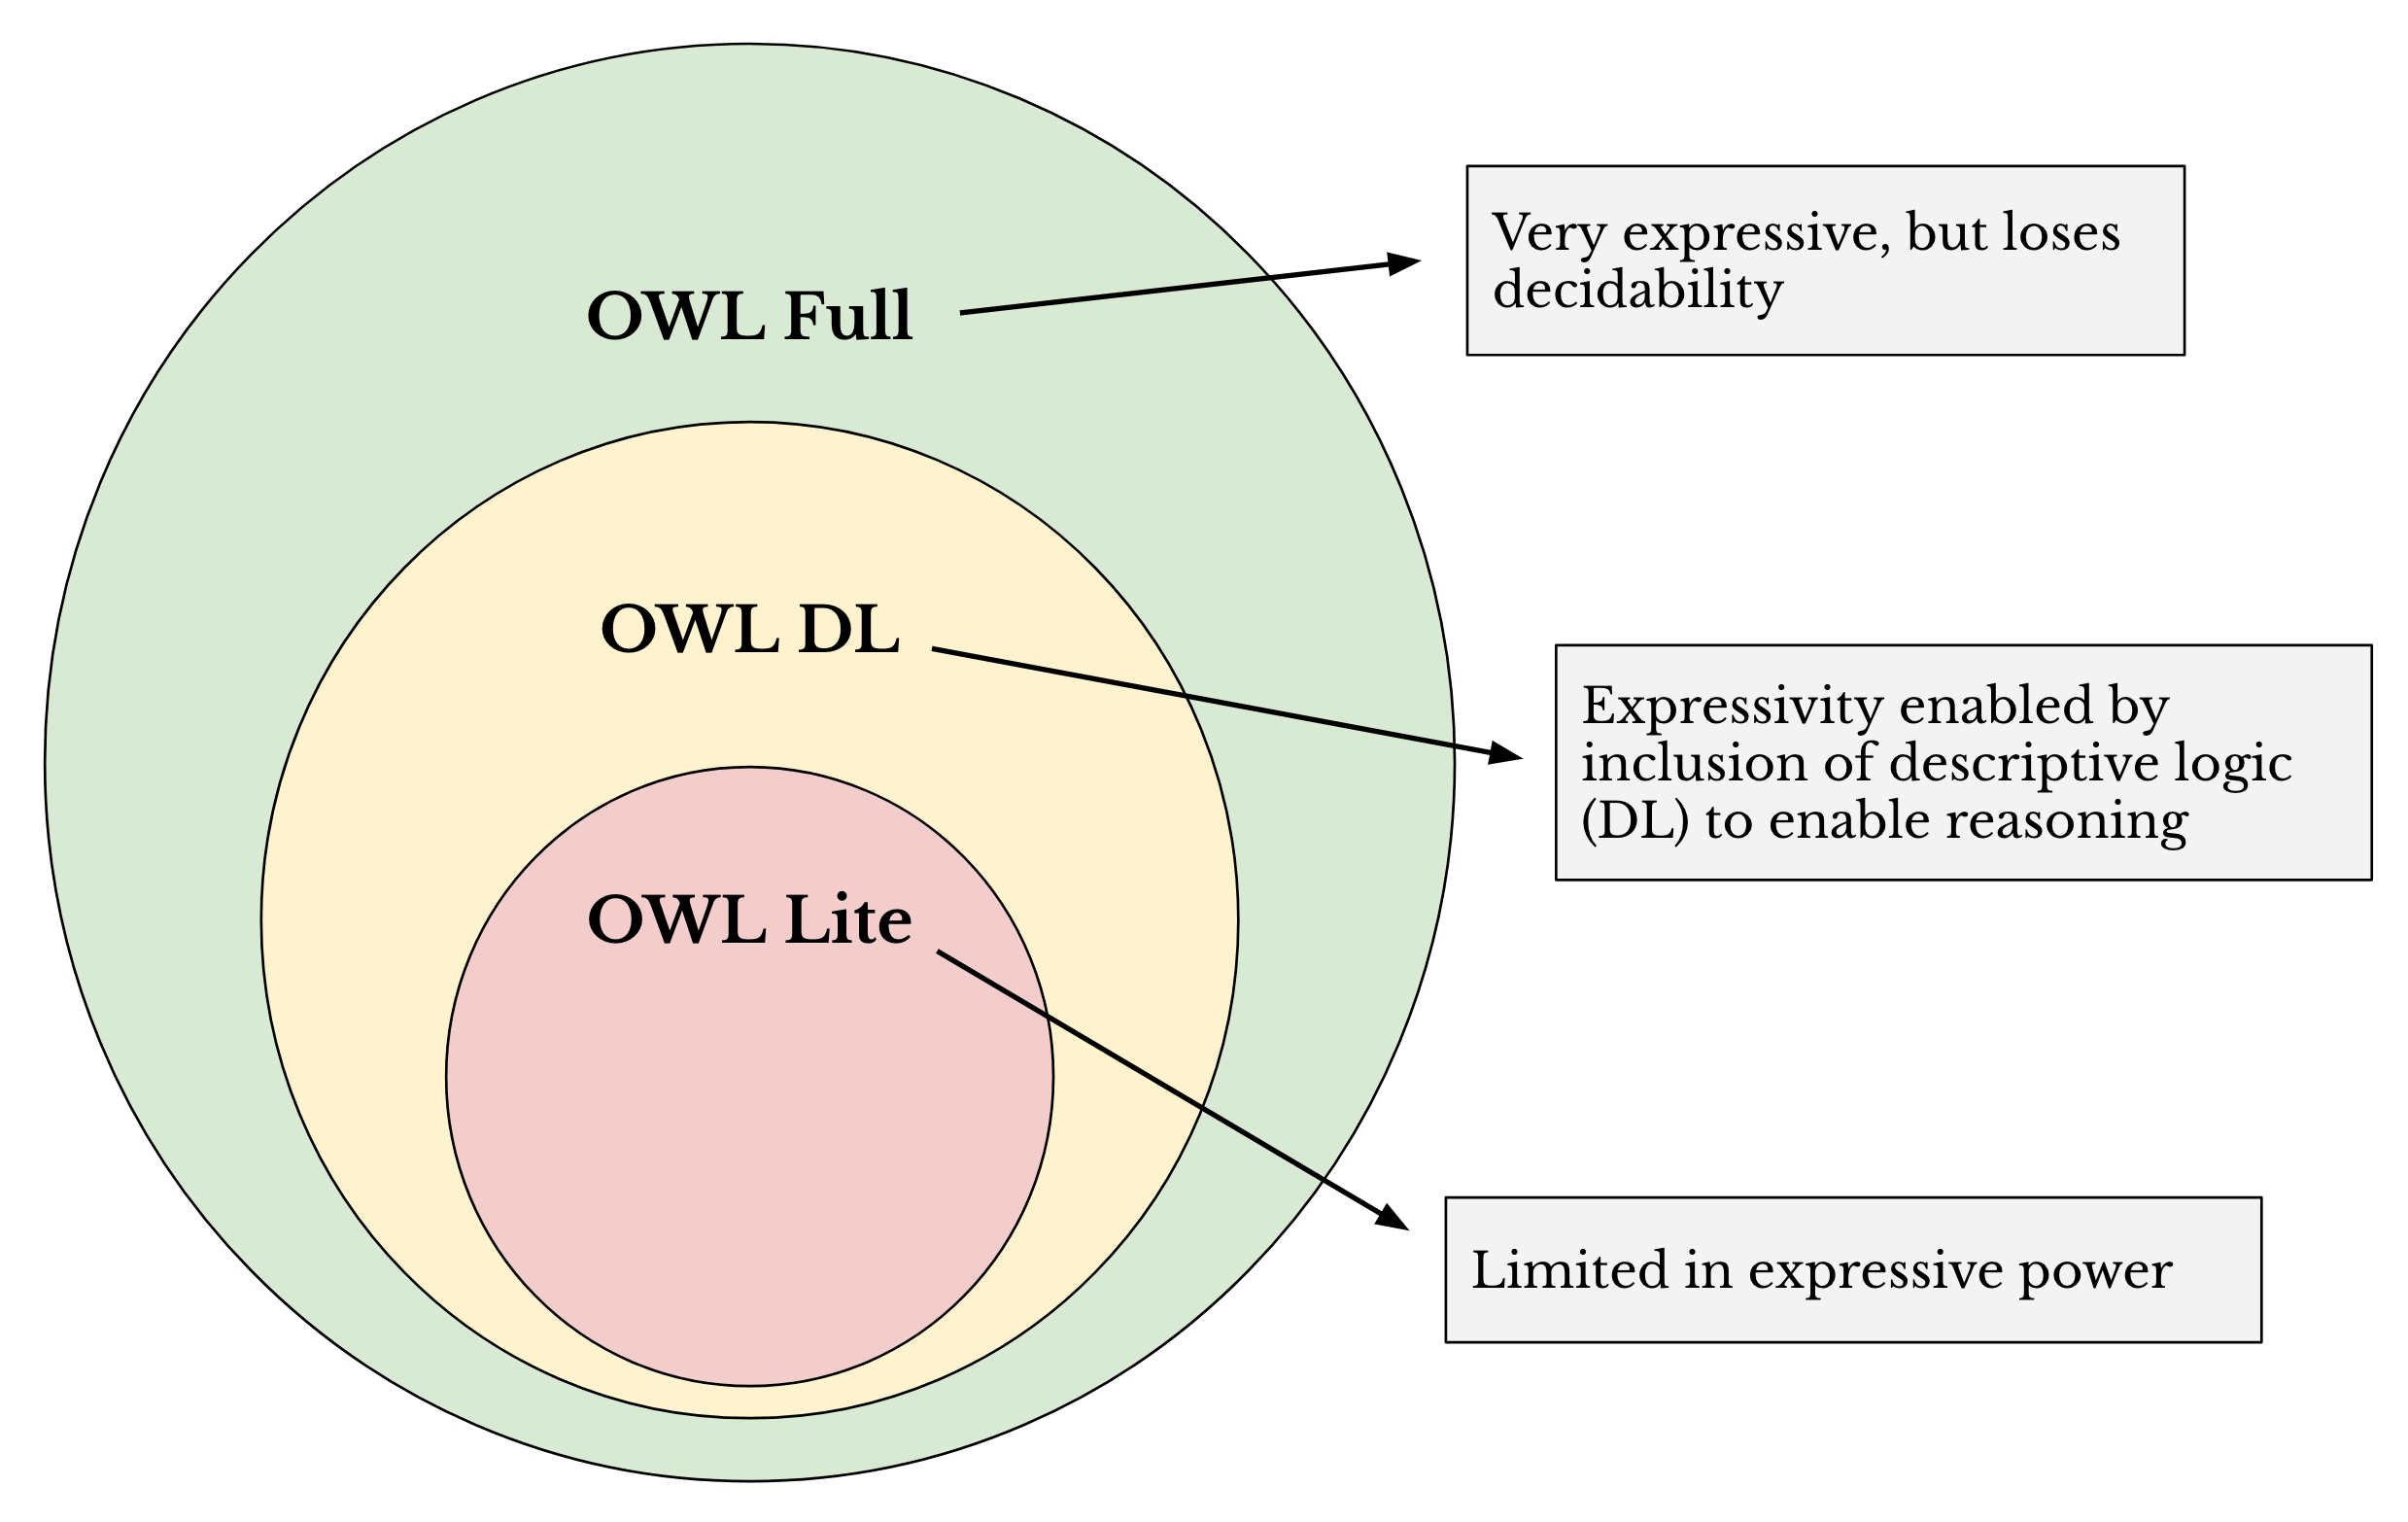
\includegraphics[width=100mm]{figures/owl_types.png}}
    \caption[Descriptive Levels of OWL]{The expressive levels of OWL ontologies. Adapted from~\cite{Marchetti2008}.}
    \label{Fig:owl_types}
\end{figure}

\subsubsection{Open Biomedical Ontologies}

As the usage of ontologies began to percolate into the biomedical domain, Ashburner and Lewis proposed the \ac{OBO} standard~\cite{Ashburner2003} to encourage the standardization of formats and identifiers, to promote openness and community feedback, and to organize information in logical units.
The OBO Foundry~\cite{Smith2007} has emerged as a central repository that has successfully supported collaboration such as the collation of several previously disparate ontologies into the Cell Line Ontology~\cite{Sarntivijai2014}.
Because the syntax of \ac{OBO} is not directly compatible with \ac{OWL}, several converters have been exist to further support the integration of \ac{OBO} with other aspects of the Semantic Web.

\subsection{Standardized Curation of Biological Pathways}

As biological knowledge is generated from experiments or extracted from the literature it must be stored in a standard format to be generally useful.
This section describes several of those formats and their applicability domains.

\subsubsection{Biological Pathways Exchange Language}

\ac{BioPAX} uses \ac{OWL} to define the conceptual knowledge in the domain of biological pathways on the molecular and cellular level.
Its ability to collect and index metabolic, signaling, molecular, gene-regulatory, and genetic interaction networks makes it an ideal exchange format for the growing number of pathway databases with varying specificities in regards to target organisms and disease indications~\cite{Demir2010}.

This was realized with the aggregation of several pathway and interaction databases (e.g., BindingDB~\cite{Gilson2016}, DrugBank~\cite{Law2014}, IntAct~\cite{Orchard2014}, \ac{KEGG}~\cite{Kanehisa2017}, Reactome~\cite{Fabregat2016}, WikiPathways~\cite{Pico2008}, etc.) to form the Pathway Commons Database~\cite{Cerami2011}.
Immediately, this database enabled exploration of molecular interactions at the highest granularity.
For example, it powers the Enrichment Map Cytoscape Plugin~\cite{Merico2010} that was used to support data-driven analysis in identifying medulloblastoma subgraphs based on intratumoral heterogeneity~\cite{Cavalli2017}.

\subsubsection{Systems Biology Markup Language}

\ac{SBML} uses a custom formalism defined with \ac{XML} to represent the dynamic and quantitative aspects of biochemical reactions, signal transduction, and gene regulatory networks~\cite{Hucka2003}.
Like \ac{BioPAX}, it provides the conceptual framework necessary to encode knowledge in the biomedical domain.
\ac{SBML} also provides the basis for CellDesigner~\cite{Funahashi2003}, which has been incredibly successful in allowing biologists without informatics backgrounds to diagram gene regulatory and biochemical networks as well as import them to graphical ordinary differential equation solvers and simulation workflows.

\subsubsection{Gene Ontology Causal Activity Models}

\acp{GOCAM} (\url{https://geneontology.cloud/docs}) combine disparate \ac{GO} annotations to generate networks of relationships between genes, their molecular functions, the biological processes in which they participate, and the cellular components in which they reside.
Relationships between genes can be expressed using terms from the Relations Ontology (\url{http://www.obofoundry.org/ontology/ro.html}) and processed using its rich set of axioms.
\acp{GOCAM} are relatively new compared to the other formats, but have the potential to provide the most standardized interpretation of the molecular interactions for which \ac{GO} is already the standard resource.

\subsubsection{Biological Expression Language}

\ac{BEL} supports the assembly of context-specific qualitative causal and correlative relations between biological entities across multiple scales.
Statements are assembled and serialized in \ac{BEL} Script with full provenance information including namespace references, relation provenance (citation and evidence), and relation metadata such as biological context (i.e. anatomy, cell, disease, etc.)~\cite{Slater2014}.
The schemata of BEL relations and BEL Scripts are depicted in Figures~\ref{fig:bel_relation} and~\ref{fig:bel_script}, respectively.

Data-driven network analyses on \ac{BEL} knowledge assemblies have been successfully performed across a wide variety of clinical applications, including the identification of upstream controllers in hepatocytes~\cite{Deehan2012}, mechanistic hypothesis generation for drug response~\cite{Laifenfeld2014}, and patient stratification~\cite{Laifenfeld2012} by using over-representation analysis techniques developed such as \ac{RCR}~\cite{Catlett2013} and pathway topological analytical methods such as \ac{NPA}~\cite{Martin2014}.

\begin{figure}
    \captionsetup{format=plain}
    \makebox[\textwidth]{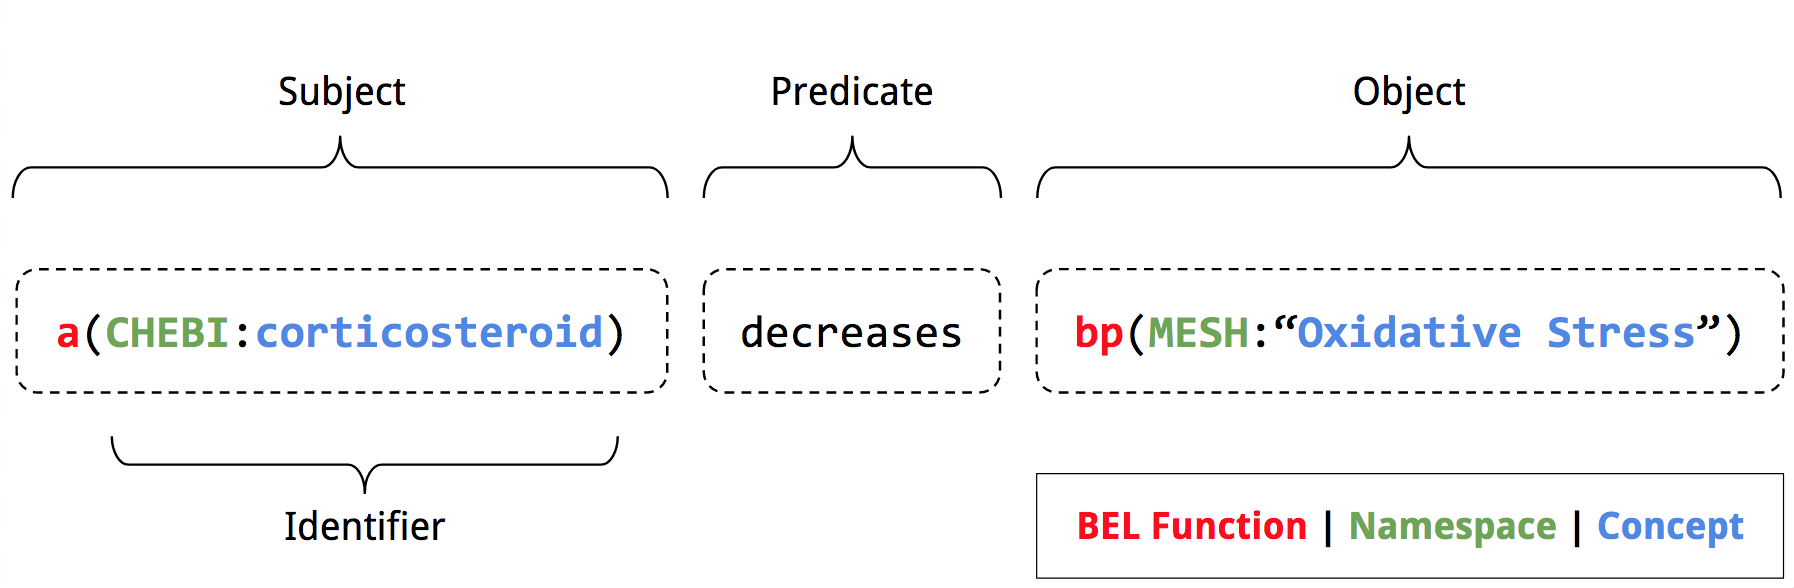
\includegraphics[width=160mm]{figures/bel_relation.png}}
    \caption[The Schema of a BEL Relation]{A BEL relation is encoded as a triplet containing a subject, a predicate, and an object. The predicate can represents the type of relation while the subject and object can either represent the abundance of molecular entities such as genes, proteins, chemicals, or more abstract concepts such as biochemical reactions, biological processes, and pathologies. Identifiers for these concepts use references to external namespaces (Figure 4B) to qualify their respective names. In this example, \ac{ChEBI}~\cite{Hastings2013} is used to qualify chemicals and \ac{MeSH}\cite{ROGERS1963} for biological processes.}
    \label{fig:bel_relation}
\end{figure}

\begin{figure}
    \captionsetup{format=plain}
    \makebox[\textwidth]{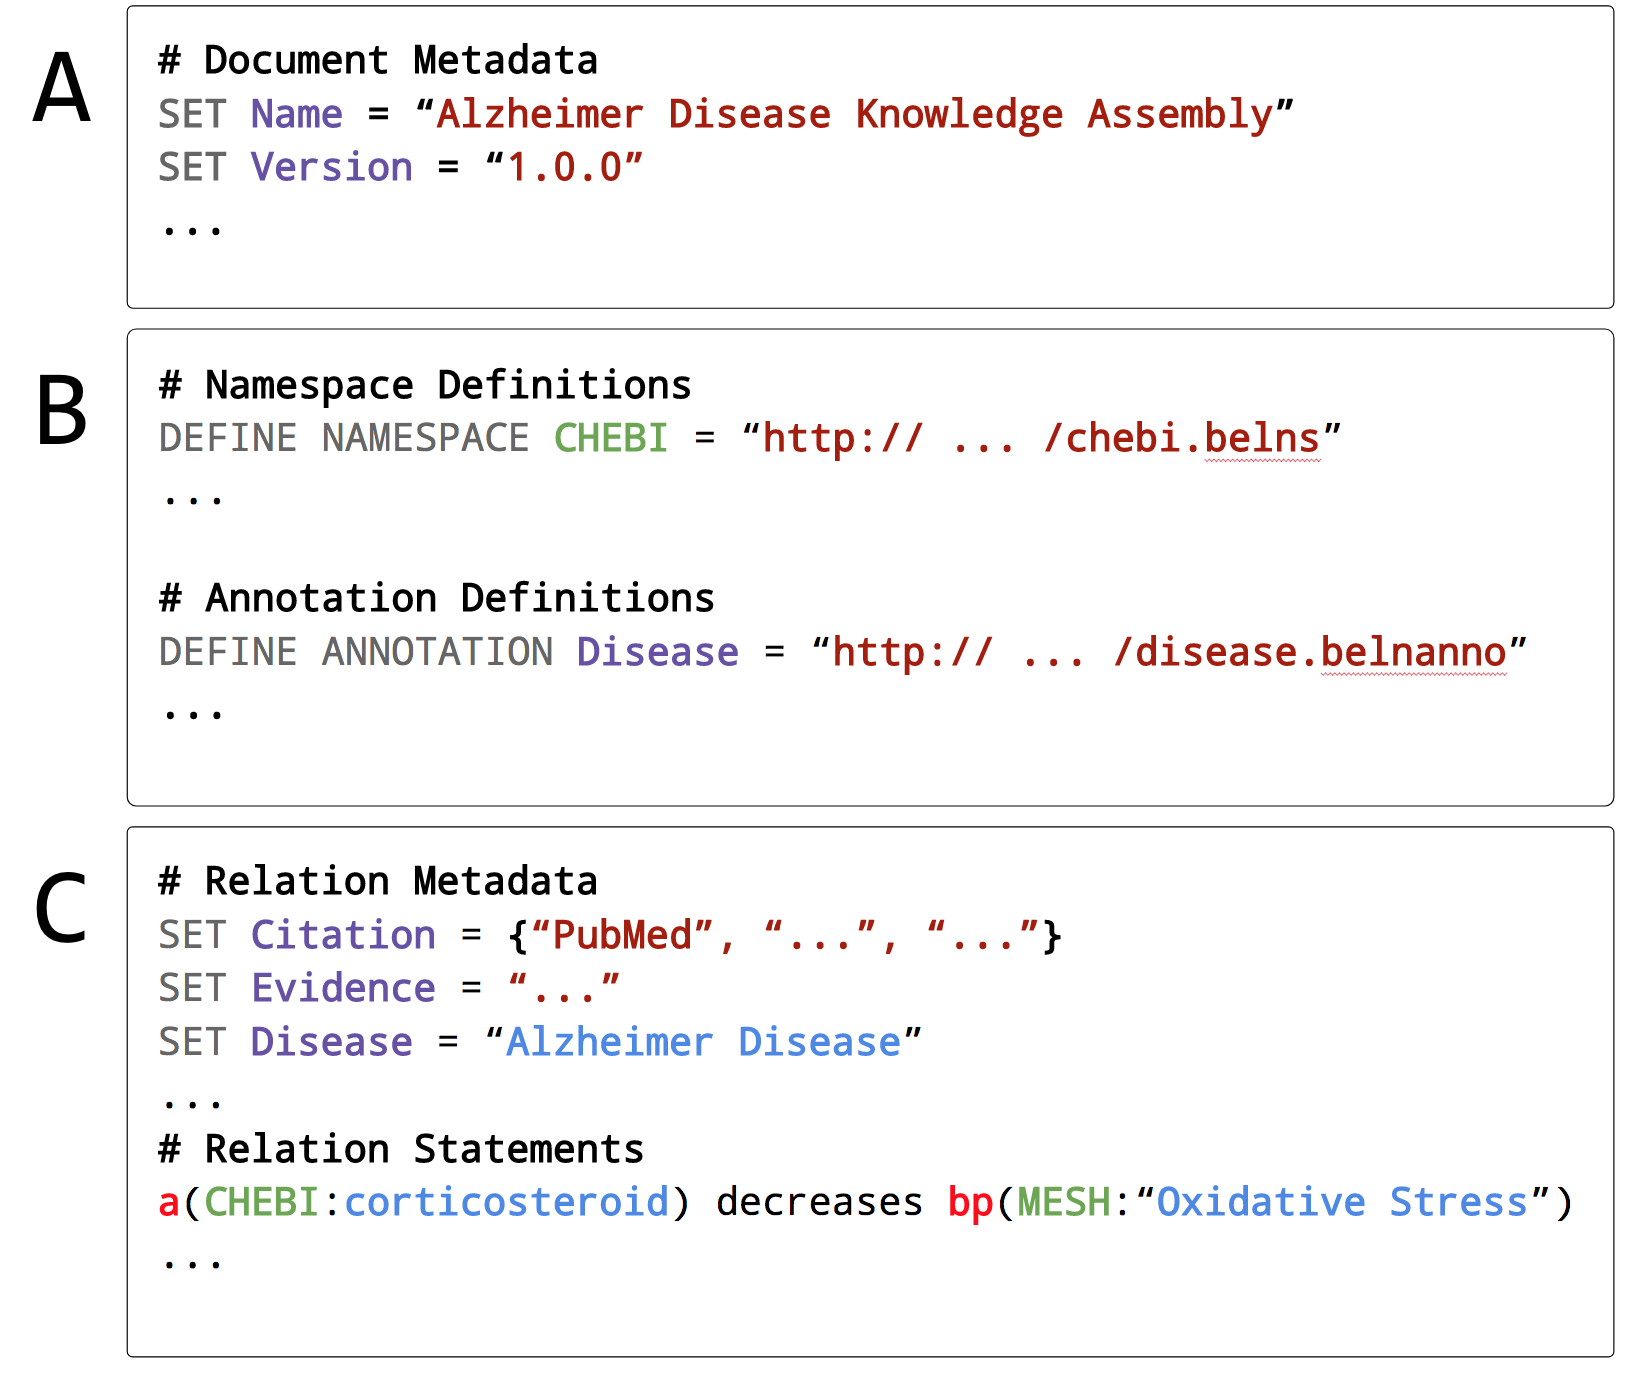
\includegraphics[scale=0.6]{figures/bel_script.png}}
    \caption[The Schema of a BEL Script]{A BEL Script contains three sections: A) the document metadata section provides provenance information such as the name, version, and author; B) the definitions section provides references to external resources that are used as identifiers and metadata in the relations section; and C) the relations section contains BEL relations and their metadata: minimally including a citation and evidence with the possibility to include additional information such as biological context (e.g., cell, anatomy, disease).}
    \label{fig:bel_script}
\end{figure}

The foray into new disease areas and clinical indications has necessitated the assembly of knowledge on wider scales from the genetic to the phenotypic and population levels.
While most modeling languages and data formats for assembling knowledge are insufficient for such a task, BEL possesses the faculty for capturing multi-scale knowledge.

In the same way \ac{BioPAX} was successful at combining many molecular pathway and interaction database, \ac{BEL} has the potential to serve as a semantic integration platform through which knowledge and data across scales can be integrated and analyzed.
\ac{BEL} can be used to reason over the previously untapped sources of chemogenomic and chemical genetic information in the realm of disease-disease, disease-protein, disease-chemical, and chemical-chemical networks.

Modeling interactions across scales is not without its issues.
As biological processes, pathologies, and phenotypes represent collections of molecular interactions, they are prone to having excessive associative and correlative relations to other biological entities.
This biases typical graph mining algorithms that rely on graph traversals to visit these types of nodes, and therefore produce less meaningful results.
While it is not within the scope of this thesis, there are many solutions for addressing these issues whose complexities vary from simple filtering to empirical traversal rules or adding extra rules for traversals.

\subsubsection{Systems Biology Graphical Notation}

\ac{SBGN}~\cite{LeNovere2009} attempts to address the inconsistency and ambiguity of current non-standardized notations for biological pathways that is problematic among \ac{BioPAX}, \ac{SBML}, \ac{BEL}, and other standardized notations.
It encompasses three variants: processes diagrams, entity relationship diagrams, and activity flow diagrams.
In a process diagram, each entity is depicted along with its transformations to other entities and the regulators of those processes.
In the entity relationship diagram, each entity appears only once and relationships are considered independent.
In the activity flow diagram, a direct presentation of the influence between entities is favored over their relationships' mechanistic underpinnings.
This variant is most related to \ac{BEL} and \acp{GOCAM}, while the others are more useful for the specific mechanistic processes that are often described in \ac{SBML} models.

\subsection{Standardized Curation of Biological Knowledge}
\label{subsec:standardized_curation}

There exists thousands of biological data databases describing different biological phenomena with varying semantics and levels of granularity (Table~\ref{tab:biological_relations}).
While many have begun to use standardized ontologies and knowledge formats, many remain.
Further, the use of standard formats does not guarantee interoperability~\cite{Domingo-Fernandez2019a}.
Integrative approaches have begun to alleviate this burden for domain-specific use cases (e.g., gene set enrichment analysis on pathway and gene set databases).
In Chapter~\ref{ch:bio2bel}, a general approach for creating integrative databases using BEL is described.

\begin{table}
    \centering
    \begin{tabular}{ r l }
        Quality & Choices \\
        \hline
        Types of Relation & Causal, Correlative, Associative, Ontological \\
        Directionality of Relation & Unidirectional or Bidirectional (reflexive) \\
        Polarity of Relation & Increases, Decreases, None \\
        Causality of Relation & Direct or Indirect \\
        Modes of Entity & Activity, Abundance, Efflux  \\
        Modifications of Entity & Post-translational modifications, gene/protein fusions, mutations \\
        States of Entity & Subcellular Location, pre-/post-conditions \\

    \end{tabular}
    \caption{Examples of qualities of biological relationships and their attributes}
    \label{tab:biological_relations}
\end{table}

Further, the quantity of knowledge in the biomedical domain is increasing at an unprecedented rate — with no signs of deceleration.
Even with the assistance of information retrieval technologies, it is overwhelming, if not impossible, for individuals or groups of researchers to be knowledgeable of the state-of-the-art in any but an incredibly specific topic.
Therefore, researchers need the assistance of automated relation extraction systems to assist in the enrichment of previously existing knowledge available and integrated from relevant, high-quality databases.

The work in this thesis makes use of an ensemble of natural language processing-based, rule-based, and machine-learning based relation extraction systems through the \ac{INDRA} interface.
References to several of its constituent general purpose and biology-specific relation extraction systems are listed in Table~\ref{tab:relation_extraction_systems}.
Additionally, a sampling of BEL-specific relation extraction systems popularized by the corresponding BioCreative V BEL Task (\url{https://biocreative.bioinformatics.udel.edu/tasks/biocreative-v/track-4-bel-task}).


\begin{table}
    \centering
    \begin{tabular}{ l l l }
        Type & Name & Reference \\
        \hline
        \multirow{4}{*}{General Purpose}
        & Eidos & \url{https://github.com/clulab/eidos} \\
        & TRIPS/CWMS & \url{http://trips.ihmc.us/parser/cgi/cwmsreader} \\
        & Hume & \url{https://github.com/BBN-E/Hume} \\
        & Sofia & \url{https://sofia.worldmodelers.com/ui/} \\
        \hline
        \multirow{8}{*}{Biology-Specific}
        & TEES & \url{https://github.com/jbjorne/TEES} \\
        & REACH & \url{https://github.com/clulab/reach} \\
        & TRIPS/DRUM & \url{http://trips.ihmc.us/parser/cgi/drum} \\
        & Sparser & \url{https://github.com/ddmcdonald/sparser} \\
        & MedScan &\cite{Novichkova2003} \\
        & RLIMS-P & \url{https://research.bioinformatics.udel.edu/rlimsp}  \\
        & ISI/AMR & \url{https://githu..com/sgarg87/big_mech_isi_gg} \\
        & Geneways &\cite{Rzhetsky2004} \\
        \hline
        \multirow{4}{*}{\ac{BEL}-Specific}
        & BELIEF &\cite{Madan2016} \\
        & BelSmile &\cite{Lai2016} \\
        & BELTracker &\cite{Rastegar-Mojarad2016} \\
        & BELMiner &\cite{Ravikumar2017} \\
    \end{tabular}
    \caption{Examples of relation extraction and reading systems with varying degrees of domain specificity}
    \label{tab:relation_extraction_systems}
\end{table}

\subsubsection{Issues with Automated Relation Extraction Systems}

Neither relation extraction systems based on rules, natural language processing, nor machine learning are without their issues.
None constitute general artificial intelligence, and thus all require maintenance and improvement to sustain their abilities to process recent scientific literature; each requires increasingly large and carefully annotated corpora to support the generation of new rules or train the extraction system to recognize new relationships.

Because relation extraction systems have many subsystems with their own subtasks, the errors from each propagate throughout.
\ac{NER} remains a difficult task due to the availability and generation of supporting ontologies that precisely describe given terms.
Though it remains unpublished and tangential to the work presented in this thesis, during the course of the curation of unstructured information outlined in Chapter~\ref{ch:recuration}, an ontology was generated to capture the complex terminology surrounding the human microtubule associated protein Tau.
It was then extended during curation of other related candidate pathophysiological mechanisms of the aetiology of \ac{AD} and named the \ac{CONSO}~(\url{https://github.com/pharmacome/terminology}).
While \ac{CONSO} formalizes the terminology and discourse from the scientific literature for protein aggregation processes in several neurodegenerative diseases (e.g., Huntington's disease, \ac{AD}, \ac{PD}), it also illustrates that the large and ongoing effort required to formalize a single area of molecular biology is not easily scaled to cover all possible biology.

Despite their recent improvements, automated relation extraction systems still omit an important aspect of systems and networks biology: the biological context.
By focusing on the sentence level, it remains difficult, if not impossible, for these systems to extract the information pertaining to the cell, cell line, tissue, model organism, disease context, or other contextual information that is crucial for the understanding of complex biology.
Even with their issues, automated relation extraction systems can be incredibly powerful when combined with manual curation in semi-automated workflows.
With careful generation of new terminologies, the inclusion of contextual information that can currently best be found by purely manual effort, and rational prioritization of automatically generated content for manual review, semi-automated workflows can make huge improvements in both the quantity, quality, and relevance of knowledge assembles.
Ultimately, these improvements lead to better downstream analysis as described in the following.
